\section{Durchführung}
\label{sec:Durchführung}
\subsection{Bestimmung des Schubmoduls $G$}
    \begin{figure}
        \centering
        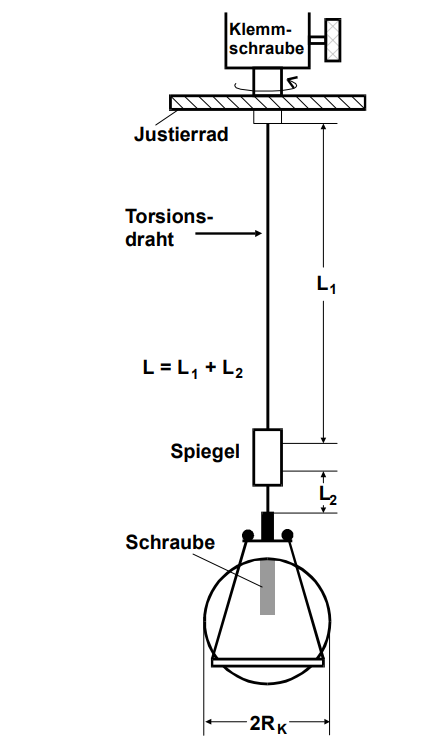
\includegraphics[height=8cm]{content/aufbau.png}
        \caption{Aufbau der Messaparatur \cite[100]{V102}.}
        \label{fig:aufbau}
    \end{figure}
    Das Schubmodul $G$ wird mittels des in des \autoref{fig:aufbau} dargestellten Aufbaus ermittelt.
    Hierzu wird die Vorrichtung durch Betätigung des Justierrades leicht ausgelenkt, so dass sie eine Drehbewegung um die eigene
    Achse vollführt. Zu Beachten ist dabei, dass die Kugel wirklich nur die Drehbewegung vollführt; andere Schwingungen können
    das Ergbenis beeinflussen und verfälschen.
    Die Schraube in der Kugel markiert die Ausrichtung des Permanentmagneten in der Kugel, dieser soll senkrecht stehen, um den
    Einfluss von diesem (besonders mit Einfluss des Erdmagnetfeldes) möglichst gering ist.
    Ein am Draht angebrachter Spiegel reflektiert drei mal pro Periode einen von einer Leuchtdiode ausgehenden Lichtstrahl auf eine
    Photodiode, welche dann ein Signal an eine digitale Schaltung übermittelt. Diese ist in \autoref{fig:schaltung} schematisch 
    dargestellt. Das erste Signal aktiviert die Zeitmessung und schaltet Flip-Flop 1 um. Das zweite 
    Signal entsteht dadurch, dass der refklektierte Strahl die Photodiode, da diese sich nicht an einem der Umkehrpunkte der Schwingung
    befindet, ein weiteres mal passiert und physikalisch somit keine Aussagekraft hat.
    Das Signal durchläuft beide Flip-Flops und schaltet diese um und wird auf diese Weise unterdrückt, sodass das dritte Signal,
    welches nach einer vollen Periode abgegeben wird, die Stoppuhr anhält und Flip-Flop 1 erneut umstellt. Die Messung ist damit abgeschlossen.
    Ein weiteres, viertes Signal setzt die Uhr mithilfe einer
    monostabilen Kippstufe zurück, wobei die Zustände der Flip-Flops ebenfalls wieder den Anfangszustand erreichen,
    sodass beim nächsten eintreffenden Signal eine weitere Messung erfolgen kann.
    Die Messaufnahme wird insgesamt zehnmal durchgeführt.
    \begin{figure}
        \centering
        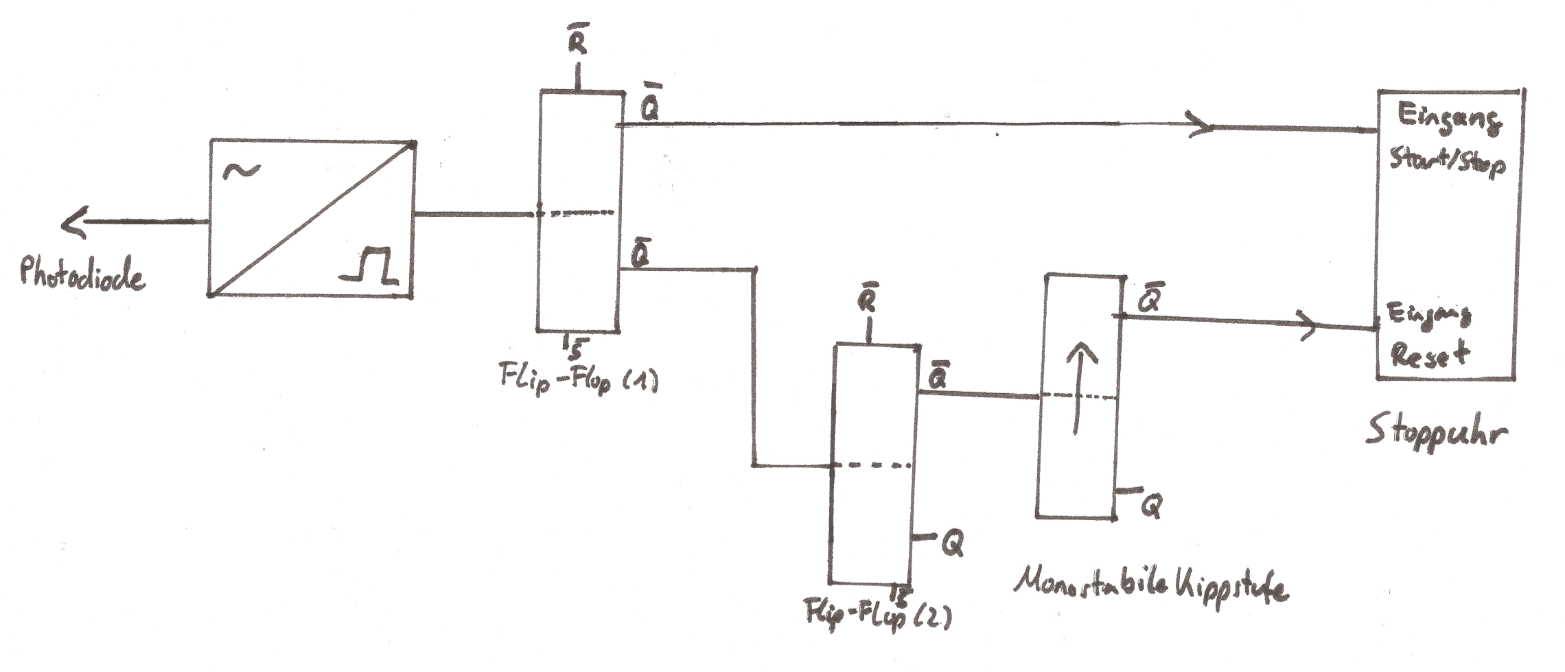
\includegraphics[width=\textwidth]{content/schaltung.png}
        \caption{Schematische Darstellung der digitalen Schaltung.}
        \label{fig:schaltung}
    \end{figure}
\subsection{Bestimmung des magnetischen Momentes} 
    Der zuvor verwendete Versuchsaufbau wird beibehalten und erweitert. Zum einen wird ein Helmholtzspulenpaar aufgestellt, welches
    an der Kugel für ein homogenes Magnetfeld sorgt, zum Anderen wird die Kugel so gedreht, dass die Schraube waagerecht ist, um
    den Einfluss des Erdmagnetfeldes zu minimieren. 
    Es wird zuerst eine Stromstärke von $0.5$A angelegt, welche in $0.5$A - Schritten bis 5A erhöht wird. Bei jeder Stromstärke
    werden insgesamt 10 Messungen durchgeführt. Hier ist es nochmal besonders wichtig auf äußere Schwingungen zu achten, da die
    Perioden immer kürzer werden mit zunehmender Stromstärke und kleine Einflüsse so vergleichsweise große Auswirkungen haben.
